\documentclass{beamer}

\usetheme{Berlin}

\usecolortheme{dolphin}

\usepackage{amsmath}
\usepackage{graphicx}
\usepackage{setspace}
\usepackage{animate}

\newcommand{\abs}[1]{\left \vert #1 \right \vert}
\newcommand{\norm}[1]{\left \Vert #1 \right \Vert}
\newcommand{\order}[1]{\mathcal{O} \left ( #1 \right )}
\newcommand{\set}[1]{\left \{ #1 \right \}}
\newcommand{\Set}[2]{\left \{ #1 \middle \vert #2 \right \}}

\newcommand{\W}[2]{W \left ( #1 ; #2 \right )}
\newcommand{\poly}[1]{\frac{x^{#1}}{(#1)!}}
\newcommand{\Poly}[1]{\frac{x^#1}{#1!}}

\newcommand{\inner}[2]{\left \langle #1, #2 \right \rangle}

\title{Introduction to Spectral Collocation}
\author{Conor McCoid}
\institute{University of Geneva}
\date{April 8th, 2019}

\begin{document}

\frame{\titlepage}

\begin{frame}

\begin{block}{The continuous problem}
$\mathcal{L} u(x) = f(x)$
\end{block}

\begin{description}
\item[$\mathcal{L}$:] Some linear operator acting on the function $u(x)$
\item[$u(x)$:] Some real-valued function (with some regularity) acting on a point $x \in \Omega \subset \mathbb{R}$
\item[$f(x)$:] Some real-valued function (with possibly different regularity than $u(x)$) acting on the same point $x$
\end{description}

\end{frame}

\begin{frame}

\begin{block}{The discrete problem}
$L_N u_N = f_N$
\end{block}

\begin{description}
\item[$L_N$:] Some operator taking $N$ pieces of information from $u_N$ and returning $N$ pieces of information in $f_N$, ie. $L_N : \mathbb{R}^N \rightarrow \mathbb{R}^N$
\item[$u_N$:] Some set of $N$ pieces of information, ie. $u_N \in \mathbb{R}^N$
\item[$f_N$:] Some set of $N$ pieces of information, ie. $f_N \in \mathbb{R}^N$
\end{description}

\end{frame}

\begin{frame}

By the description of the discrete problem $L_N$ is some matrix of size $N \times N$ and $u_N$ and $f_N$ are both vectors of length $N$.
The solution vector $u_N$ is then $u_N = L_N^{-1} f_N$.

~

We want our solution vector $u_N$ to correspond in some way to the solution function of the continuous problem.
That is, we want
\begin{equation*}
\lim_{N \to \infty} u_N \equiv u(x)
\end{equation*}
in some sense.

% At this stage it would be helpful to draw a diagram, showing the discrete spaces inside the continuous ones and how the projection would work
\end{frame}

\begin{frame}

The discrete space may be defined by a set of basis functions (called \textit{trial functions}), $\set{\phi_k(x)}_{k=1}^N$.
Our approximation $u_N$ then defines a linear combination of these functions:
\begin{equation*}
u_N \equiv \sum_{k=1}^N a_k \phi_k(x) .
\end{equation*}

\end{frame}

\begin{frame}

We want now that when we apply $\mathcal{L}$ to this linear combination, we'll retrieve an approximation to $f(x)$:
\begin{equation*}
\sum_{k=1}^N a_k \mathcal{L} \phi_k(x) \approx f(x) .
\end{equation*}
More specifically, we want that
\begin{equation*}
\inner{\sum_{k=1}^N a_k \mathcal{L} \phi_k(x) - f(x) }{\psi_j(x) } = 0 \ \forall j=1,...,N
\end{equation*}
for some inner product defined on the space of functions and for some set of \textit{test functions} $\psi_j(x)$.

\end{frame}

\begin{frame}
This allows us to choose three things:
\begin{itemize}
\item the inner product $\inner{\cdot}{\cdot}$,
\item the trial functions $\phi_k(x)$,
\item and the test functions $\psi_j(x)$.
\end{itemize}

Different sets of these choices lead to different classes of methods.
\end{frame}

\begin{frame}

\begin{block}{Finite Element Methods}
$\phi_k(x)$ and $\psi_j(x)$ have finite support (locally defined).
\end{block}
~
\begin{block}{Spectral Methods}
$\phi_k(x)$ and $\psi_j(x)$ have infinite support (globally defined).
\end{block}
% main difference, not only difference
\end{frame}

\begin{frame}

\begin{block}{Galerkin}
The trial functions individually satisfy the boundary conditions.
\end{block}

\begin{block}{Tau} % I don't think this is right
$\inner{\phi_k(x)}{\psi_j(x)} = \begin{cases} 1 & k = j \\ 0 & k \neq j \end{cases} $
\end{block}

\begin{block}{Collocation}
$\inner{\phi_k(x)}{\psi_j(x)} = \phi_k(x_j)$
\end{block}
% not exactly their definitions but they'll give us the right idea
\end{frame}

\begin{frame}
\begin{description}
\item[Galerkin] $u_N$ contains the coefficients in the \textit{Galerkin basis}.
\item[Tau] $u_N$ also contains coefficients, but for a more general basis.
\item[Collocation] $u_N$ contains the values of the approximation at some set of \textit{collocation points}, $u_N(x_j)$.
\end{description}
\end{frame}

\begin{frame}

We will focus on spectral collocation (global basis functions, minimize residual point by point).
That is,
\begin{equation*}
L_N \begin{bmatrix}
u_N(x_1) \\ u_N(x_2) \\ \vdots \\ u_N(x_N)
\end{bmatrix} = \begin{bmatrix}
f(x_1) \\ f(x_2) \\ \vdots \\ f(x_N)
\end{bmatrix}
\end{equation*}
with $L_N$ being a matrix representing the linear operator.

~

We need to know $L_N$ to solve this system.
For that, we need to know the differentiation matrix, $D_N$.

\end{frame}

\begin{frame}

$D_N$ must work perfectly for the trial functions, $\phi_k(x)$:
\begin{equation*}
D_N \begin{bmatrix}
\phi_k(x_1) \\ \phi_k(x_2) \\ \vdots \\ \phi_k(x_N)
\end{bmatrix} = \begin{bmatrix}
\phi_k'(x_1) \\ \phi_k'(x_2) \\ \vdots \\ \phi_k'(x_N)
\end{bmatrix}
\end{equation*}
for all $k = 1,...,N$.

~

$D_N$ is singular since $D_N \begin{bmatrix} 1 & 1 & \dots & 1 \end{bmatrix}^\top = 0$ (nilpotent, actually).
The matrix representing second order differentiation is the square of $D_N$.
Likewise, $D^{(m)}_N = D^m_N$.
% you can think of D_N like you would a finite difference matrix: it performs differentiation on functions defined on a given set of points
\end{frame}

\begin{frame}

\begin{block}{The continuous operator}
\begin{equation*}
\mathcal{L} u(x) = u^{(m)}(x) + \sum_{k=1}^m p_k(x) u^{(m-k)}(x)
\end{equation*}
\end{block}
\begin{block}{The discrete operator}
\begin{equation*}
L_N = D^m_N + \sum_{k=1}^m P_k D^{m-k}_N
\end{equation*}
where $P_k$ is a $N \times N$ diagonal matrix with entries $p_k(x_j)$.
\end{block}

\end{frame}

\begin{frame}
$L_N$ is singular because $D_N$ and all of its powers are singular.
Boundary conditions are needed to make $L_N$ nonsingular.
The number of BCs matches the order of the problem, $m$.

~

BCs may be concatenated so the system is overdetermined or they can be used to replace rows in $L_N$.
\end{frame}

\begin{frame}

What should we choose for $\phi_k(x)$?
\begin{itemize}
\item $\phi_k(x)$ span a finite dimensional space
\item they should be orthogonal with respect to some inner product (generally a weighted $L_2$ inner product)
\item they can be used to approximate functions in the infinite space arbitrarily well
\end{itemize}

Some candidates:
\begin{itemize}
\item Sinusoids (Fourier series)
\item Polynomials (Weierstrass approximation theorem)
\end{itemize}

\end{frame}

\begin{frame}

\frametitle{Jacobi polynomials}

\begin{align*}
& P_n^{(\alpha, \beta)}(x) = \\
& \frac{\Gamma(\alpha + n + 1)}{n! \Gamma(\alpha + \beta + n + 1)} \sum_{m=0}^n \binom{n}{m} \frac{\Gamma(\alpha + \beta + n + m + 1)}{\Gamma(\alpha + m + 1)} \left ( \frac{x-1}{2} \right )^m
\end{align*}

Orthogonal with respect to the weight $(1-x)^\alpha (1+x)^\beta$ on $[-1,1]$

\end{frame}

\begin{frame}

\frametitle{Ultraspherical polynomials}

Special cases of the Jacobi polynomials with $\alpha = \beta$

\begin{block}{Legendre polynomials}
$\alpha = \beta = 0$
\end{block}

\begin{block}{Chebyshev polynomials}
$\alpha = \beta = 1/2$
\end{block}

\end{frame}

\begin{frame}

\frametitle{Sturm-Liouville Theory}

The Sturm-Liouville Problem (SLP):
\begin{equation*}
\mathcal{L}_{SL} \phi(x) = -\left ( p(x) \phi'(x) \right )' + q(x) \phi(x) = \lambda w(x) \phi(x)
\end{equation*}
with $p \in C^1(-1,1)$, $p>0$, $q, w \geq 0$, $q, w \in C[-1,1]$.

~

If $\mathcal{L}_{SL}$ is self-adjoint ($\inner{\mathcal{L}_{SP}u}{v} = \inner{u}{\mathcal{L}_{SP}v}$) then the SLP has a countable number of eigenvalues ($\lambda$) and the eigenfunctions ($\phi(x)$) form a complete set in $L^2(-1,1)$ and $L_w^2(-1,1) = \Set{u \in L^2(-1,1)}{\int_{-1}^1 u^2 w dx < \infty}$.
% in essence, the functions phi(x) make great candidates for our basis functions
\end{frame}

\begin{frame}

\begin{block}{Projection of $u(x) \in L_w^2(-1,1)$}
\begin{equation*}
P_N u(x) = \sum_{k=1}^N \hat{u}_k \phi_k(x)
\end{equation*}
where $\hat{u}_k = \int_{-1}^1 \phi_k(x) u(x) w(x) dx / \lambda_k$
\end{block}

~

If $p(\pm 1) = 0$ and $u \in C^\infty(-1,1)$ then $\abs{\hat{u}_k} \to 0$ faster than any polynomial power of $1/k$ (known as spectral convergence).

\end{frame}

\begin{frame}

Special cases of SLP: ultraspherical polynomials
\begin{itemize}
\item $p(x) = (1-x^2)^{\alpha+1}$
\item $q(x) =c(1-x^2)^\alpha$
\item $w(x) = (1-x^2)^\alpha$
\end{itemize}
For $\alpha = 0$ the eigenfunctions are the Legendre polynomials.
For $\alpha = 1$ the eigenfunctions are the Chebyshev polynomials.

\end{frame}

\begin{frame}

\frametitle{Legendre polynomials}

\begin{block}{Rodrigues' formula}
\begin{equation*}
P_n(x) = \frac{1}{2^n n!} \frac{d^n}{dx^n} (x^2-1)^n
\end{equation*}
\end{block}

\begin{figure}
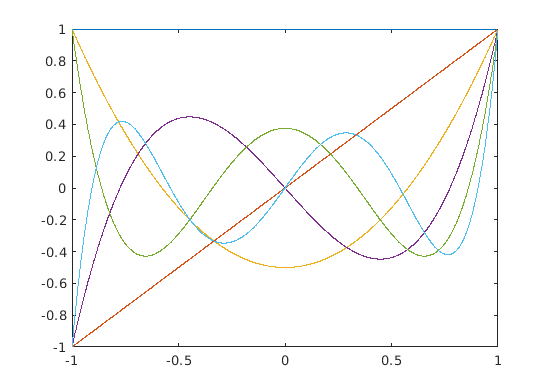
\includegraphics[width=0.5\textwidth]{legendreP.png}
\end{figure}

\end{frame}

\begin{frame}

\frametitle{Chebyshev polynomials}

\begin{block}{Closed form}
\begin{equation*}
T_n(x) = \cos \left ( n \arccos \left ( x \right ) \right )
\end{equation*}
\end{block}

\begin{figure}
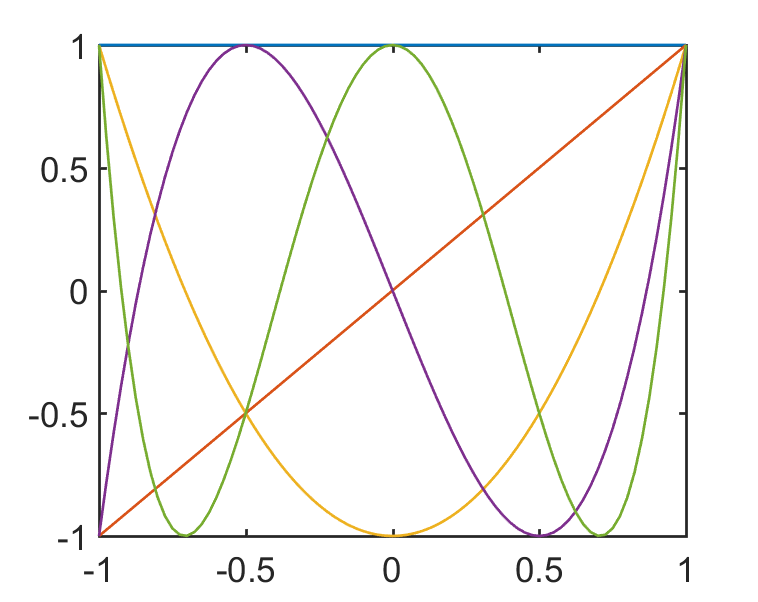
\includegraphics[width=0.5\textwidth]{ChebPoly.png}
\end{figure}

\end{frame}

\begin{frame}

\begin{block}{Weighted Gaussian quadrature}
\begin{equation*}
\int_{-1}^1 f(x) w(x) dx = \sum_{k=1}^N w_k f(x_k)
\end{equation*}
\end{block}

~

We use the points $x_k$ as our collocation points.
The weight function $w(x)$ is used in the weighted inner product
$
\inner{\cdot}{\cdot}_w .
$

\end{frame}

\begin{frame}

\begin{description}
\item[Gauss-Jacobi:] $w(x) = (1-x)^\alpha (1+x)^\beta$
\item[Gauss-Legendre:] $w(x) = 1$
\item[Chebyshev-Gauss:] $w(x) = \sqrt{1-x^2}$
\end{description}

~

The corresponding polynomials are orthogonal both with respect to $\inner{\cdot}{\cdot}_w$ and the quadrature rule.
%explain this more clearly in words

\end{frame}

\begin{frame}

\frametitle{A good choice}

\begin{block}{Chebyshev polynomials}
\begin{equation*}
T_n(x) = \cos \left ( n \arccos \left ( x \right ) \right )
\end{equation*}
\end{block}

\begin{block}{Chebyshev-Gauss(-Lobatto) quadrature}
\begin{equation*}
\int_{-1}^1 f(x) \sqrt{1-x^2} dx = \sum_{k=0}^N w_k f \left ( \cos \left ( \frac{ k \pi}{N} \right ) \right )
\end{equation*}
\end{block}

\end{frame}

\begin{frame}

So our trial functions are $T_n(x)$, the Chebyshev functions and our collocation points are $x_k = \cos \left ( \frac{k \pi}{N} \right )$, the Chebyshev points.
The differentiation matrix $D_N$ is then:
\begin{figure}
\includegraphics[width=0.5\textwidth]{ChebDiffMat.pdf}
\end{figure}

% point out each element is defined explicitly
\end{frame}

\begin{frame}
$u''(x) - u(x) = \cos(\pi x / 2)$, $u(\pm 1) = 0$, $u(x) = -\cos(\pi x/2) / ( (\pi/2)^2 + 1)$
\begin{figure}
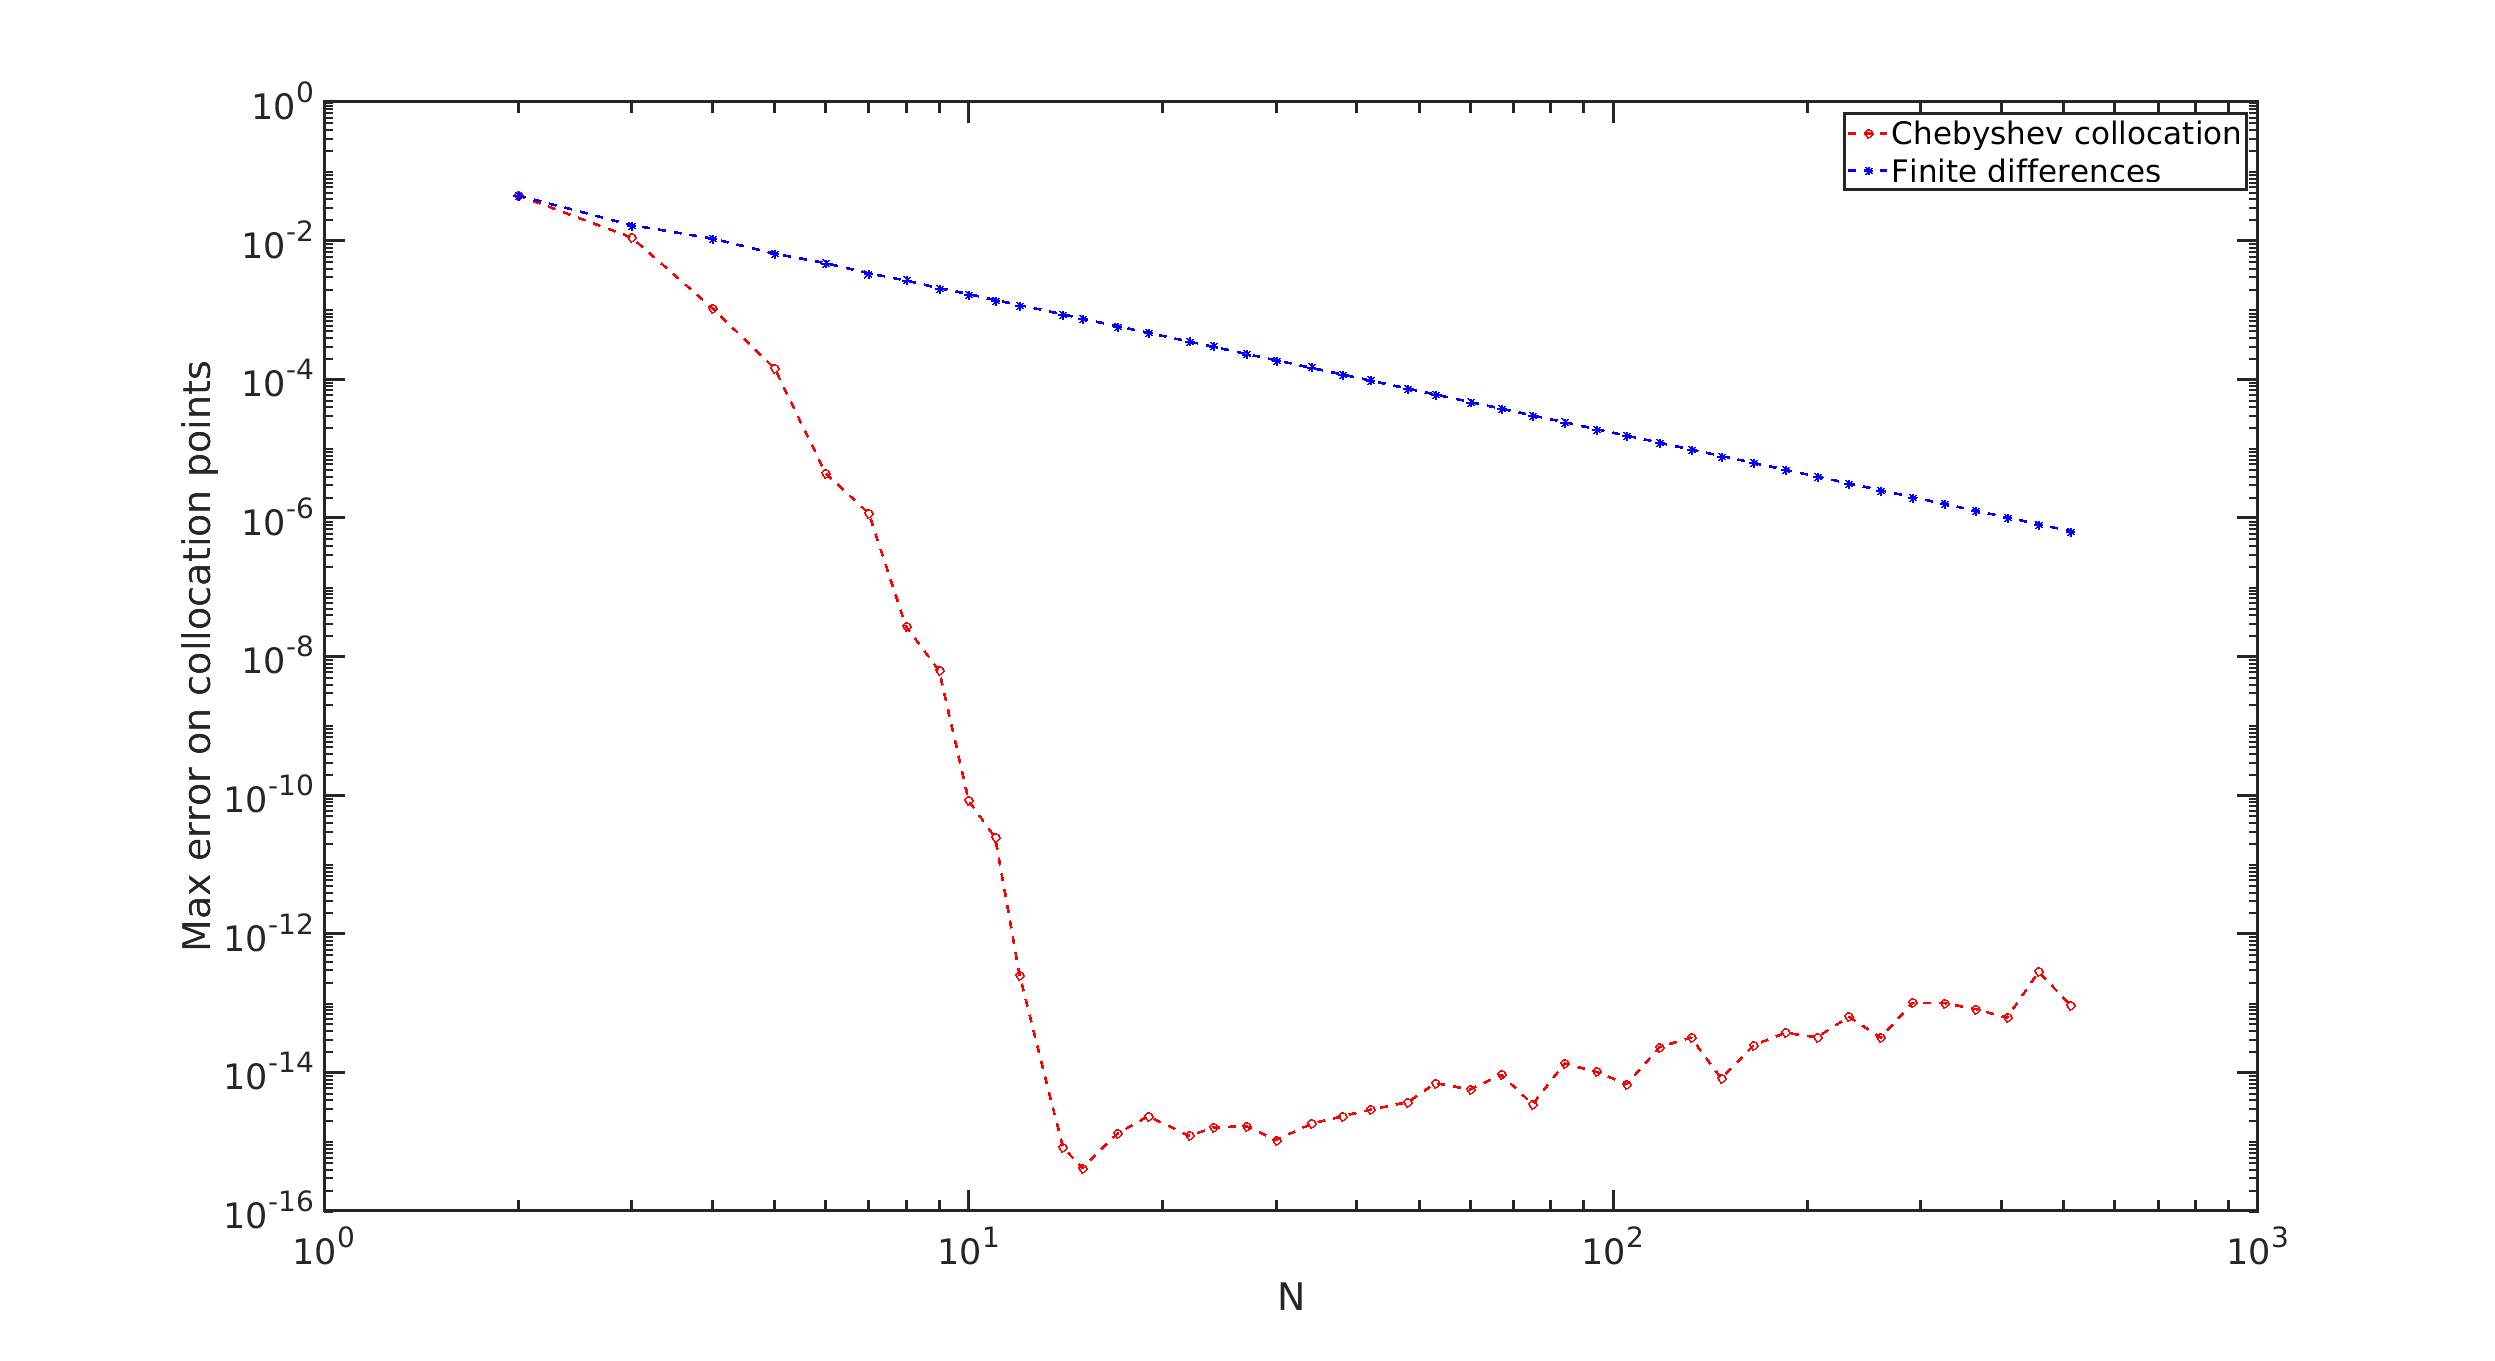
\includegraphics[width=\textwidth]{example_seminar1.png}
\end{figure}
% comparison of collocation v finite diff solving a linear ode
% point out (by drawing on board) the error behaviour: spectral convergence of approximation, linear increase of round-off error
\end{frame}

% we want to reduce this round-off error by eliminating the need to perform a matrix system solve
% that is, we want to find the inverse of the matrix LN

\begin{frame}
\frametitle{$L_N L_N^{-1} = I$}
Let $R_j$ be the $j$--th column of $L_N^{-1}$.
% this column is a vector of N+1 values, just like the vectors uN and fN, which represent functions
% so we can think of Rj as a function
\begin{equation*}
\mathcal{L} R_j(x_i) = \begin{cases} 1 & i = j \\ 0 & i \neq j \end{cases}
\end{equation*}
% there's also a number of boundary conditions we need to consider, but for now we'll ignore them
% There's also the question of the rows we removed to make LN invertible
% we'll use this ansatz to find Rj(x)
\begin{equation*}
R_j(x) = \sum_{k=1}^m G_{k,j}(x) P_k(x)
\end{equation*}
where $\mathcal{L} P_k(x) = 0$.
\end{frame}

\begin{frame}
% to find what both G and P need to be, we use variation of parameters
\begin{block}{Variation of parameters}
\begin{equation*}
\sum_{k=1}^m G_{k,j}'(x) P_k^{(n)}(x) = 0, \quad n = 0,...,m-2
\end{equation*}
\end{block}
% do the steps between these two lines on the board?
\begin{equation*}
\implies \mathcal{L} R_j(x) = \sum_{k=1}^m G_{k,j}'(x) P_k^{(m-1)}(x)
\end{equation*}
% evaluating this at a point xi we need this to be zero unless i equals j
\end{frame}

\begin{frame}
% so we need these conditions on G
\begin{equation*}
\implies G_{k,j}'(x_i) = \begin{cases} \beta_{k,j} & i = j \\ 0 & i \neq j \end{cases}
\end{equation*}
% then we need the beta coefficients to satisfy these conditions
\begin{equation*}
\implies \sum_{k=1}^m \beta_{k,j} P_k^{(n)}(x_j) = \begin{cases} 1 & n = m-1 \\ 0 & n = 0,...,m-1 \end{cases}
\end{equation*}
% which may be represented by the system
\begin{equation*}
\implies \begin{bmatrix} P_1(x_j) & \dots & P_m(x_j) \\ \vdots & & \vdots \\ P_1^{(m-1)}(x_j) & \dots & P_m^{(m-1)}(x_j) \end{bmatrix} \begin{bmatrix} \beta_{1,j} \\ \vdots \\ \beta_{m,j} \end{bmatrix} = \begin{bmatrix} 0 \\ \vdots \\ 0 \\ 1 \end{bmatrix}
\end{equation*}
% the conditons on G we know how to satisfy, though I won't go into the details
% one thing to note though is that there is one point for each Gkj that cannot be made to satisfy these conditions
% these points come from the row removal and form a set V
\end{frame}

\begin{frame}
% so for each Gkj there is a point vk where Gkj' is nonzero but should be
% to make sure all the right conditions are still satisfied, we need the functions Pk to satisfy
\begin{equation*}
P_k^{(n)}(v_k) = \begin{cases} 1 & n = 1 \\ 0 & n = 0,...,m-2 \end{cases}
\end{equation*}
% so we need a specific set of homogeneous solutions to the linear operator
% suppose we don't have this set but we do have another, then we can construct this set by taking a linear combination
\begin{equation*}
P_k(x) = \sum_{n=1}^m \gamma_{k,n} \hat{P}_n(x)
\end{equation*}
% then the conditions on Pk and the form it takes gives us a nearly identical system to the one for beta
\begin{equation*}
\implies \begin{bmatrix} \hat{P}_1(v_k) & \dots & \hat{P}_m(v_k) \\ \vdots & & \vdots \\ \hat{P}_1^{(m-1)}(v_k) & \dots & \hat{P}_m^{(m-1)}(v_k) \end{bmatrix} \begin{bmatrix} \gamma_{k,1} \\ \vdots \\ \gamma_{k,m} \end{bmatrix} = \begin{bmatrix} 0 \\ \vdots \\ 0 \\ 1 \end{bmatrix}
\end{equation*}
\end{frame}

\begin{frame}
% the matrices of these systems are special, and are called fundamental matrices
\begin{block}{Fundamental matrix and Wronskian}
\begin{equation*}
\det \left ( \begin{bmatrix} f_1(x) & \dots & f_m(x) \\ \vdots & & \vdots \\ f_1^{(m-1)}(x) & \dots & f_m^{(m-1)}(x) \end{bmatrix} \right ) = \W{\set{f_k}_{k=1}^m}{x}
\end{equation*}
\end{block}
% we can use Cramer's rule to get the values of gamma and beta
\begin{equation*}
\implies \gamma_{k,n} = (-1)^{n+m} \frac{ \W{\set{\hat{P}_i}_{i \neq n}}{v_k} }{ \W{\set{\hat{P}_i}_{i=1}^m}{v_k} }
\end{equation*}
% generally the Wronskians are a challenge to compute, so this doesn't help us immediately
\end{frame}

\begin{frame}
% note, however, that the fundamental matrix in P is a product of the fundamental matrix in hatP times the matrix of gamma coefficients
\begin{align*}
& \begin{bmatrix} P_1(x) & \dots & P_m(x) \\ \vdots & & \vdots \\ P_1^{(m-1)}(x) & \dots & P_m^{(m-1)}(x) \end{bmatrix} \\
& = \begin{bmatrix} \hat{P}_1(x) & \dots & \hat{P}_m(x) \\ \vdots & & \vdots \\ \hat{P}_1^{(m-1)}(x) & \dots & \hat{P}_m^{(m-1)}(x) \end{bmatrix} \begin{bmatrix} \gamma_{1,1} & \dots & \gamma_{m,1} \\ \vdots & & \vdots \\ \gamma_{1,m} & \dots & \gamma_{m,m} \end{bmatrix}
\end{align*}
% (write this in a simplified form on the board: P beta = hatP Gamma beta = [0 ... 1] -> beta = Gamma^-1 hatP^-1 [0 ... 1]
% so if we can find the Wronskian for the fundamental solution set we know then we can get it for the set we don't know very easily
\end{frame}

\begin{frame}
% so when are the Wronskians easy to find? for constant coefficient linear operators
\begin{block}{Constant coefficient linear operators}
$\mathcal{L} u(x) = u^{(m)}(x) + \sum_{k=1}^m a_k u^{(m-k)}(x)$
\end{block}
% the fundamental solution set of these operators is polynomials times exponentials
\begin{equation*}
\hat{P}_{k,j}(x) = \Poly{j} e^{\lambda_k x}
\end{equation*}
where $\lambda_k$ is a root with multiplicity $m_k$ ($\sum m_k = m$) of the polynomial with coefficients $a_k$ and $j = 0,...,m_k-1$.
\end{frame}

% the fundamental matrix for such a set has a very specific form (draw on board, incl. the matrix Omega and the pieces Fk(x))
% the inverses of the Fk(x) must be upper triangular and toeplitz since Fk(x) are
% then we only need the last column of Fk(x)^-1 to get all of it, and for that we only need the Wronskians of consecutive polynomials (present without proof)
% so to get the inverse(s) of hatP we need only the following procedure (on board)

% for the boundary conditions we add constants to Gkj, which doesn't change any of our results since they depend only on Gkj'
% then we solve for these constants in a brute force fashion to get Rj to satisfy the BCs

\begin{frame}
$u''(x) - u(x) = \cos(\pi x / 2)$, $u(\pm 1) = 0$, $u(x) = -\cos(\pi x/2) / ( (\pi/2)^2 + 1)$
\begin{figure}
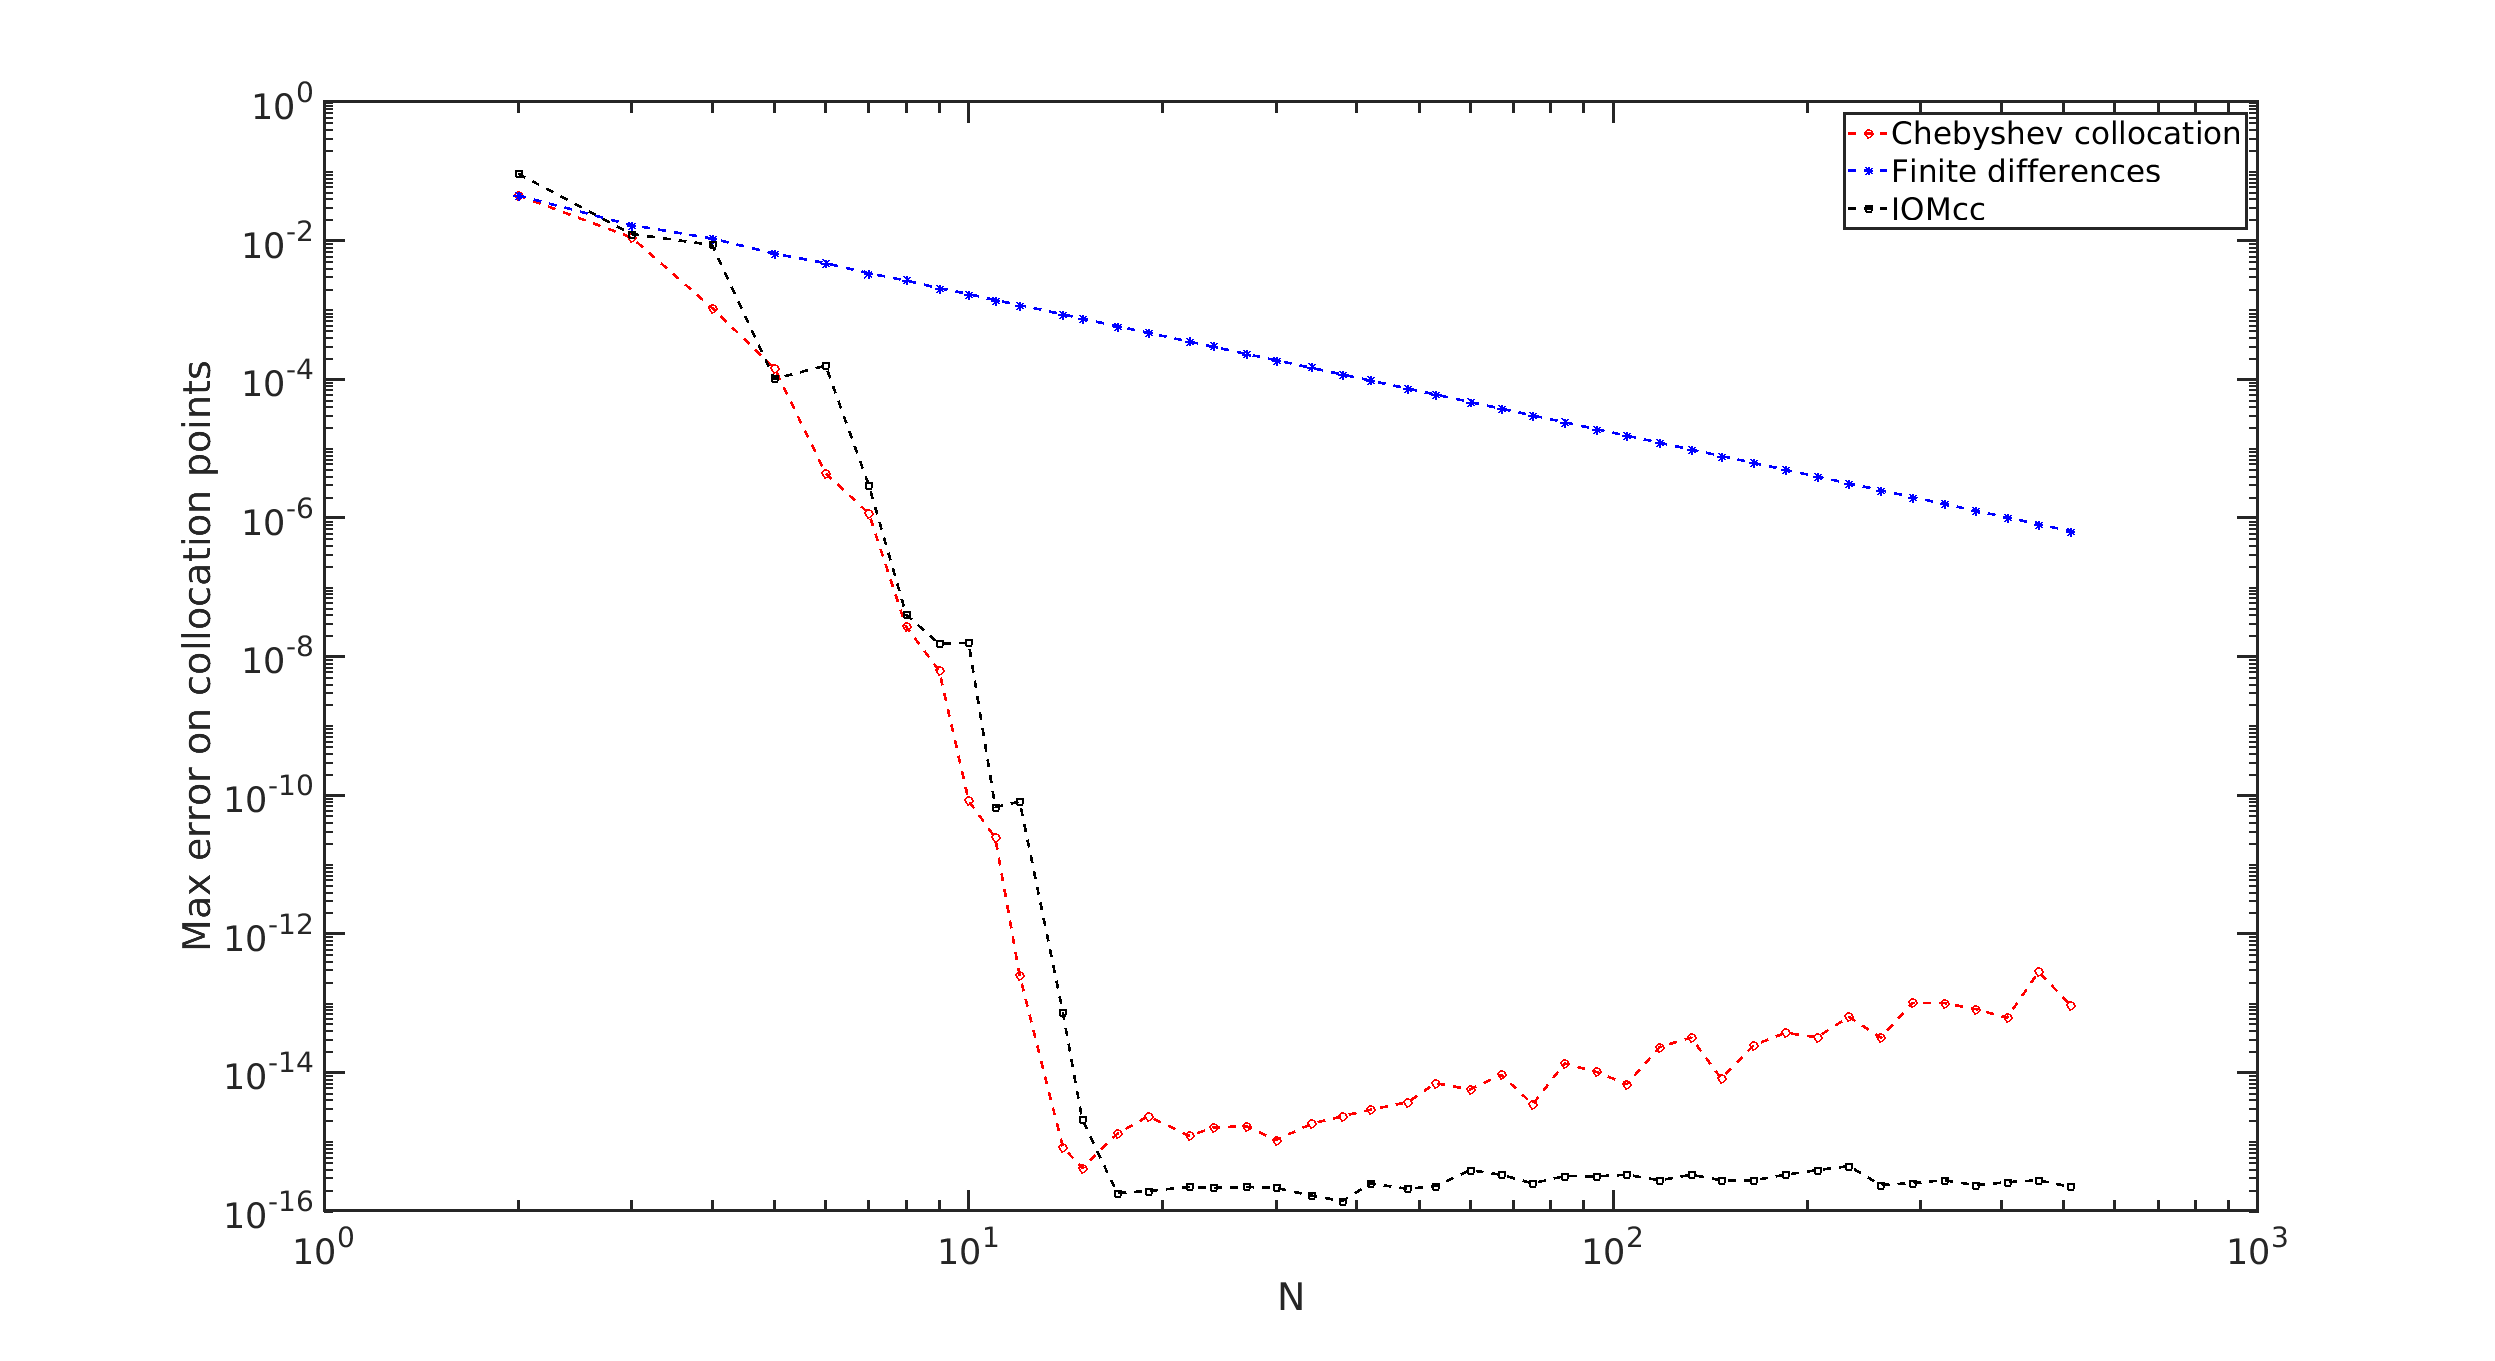
\includegraphics[width=\textwidth]{example_seminar2.png}
\end{figure}
\end{frame}

\end{document}